
\documentclass[border=8pt]{standalone}

% Core packages
\usepackage{tikz}
\usepackage{ragged2e}
\usetikzlibrary{arrows.meta,backgrounds,fit,matrix,positioning}

% Paragraphs
\setlength{\parindent}{0pt}
\setlength{\parskip}{1\baselineskip}

\begin{document}
\scriptsize
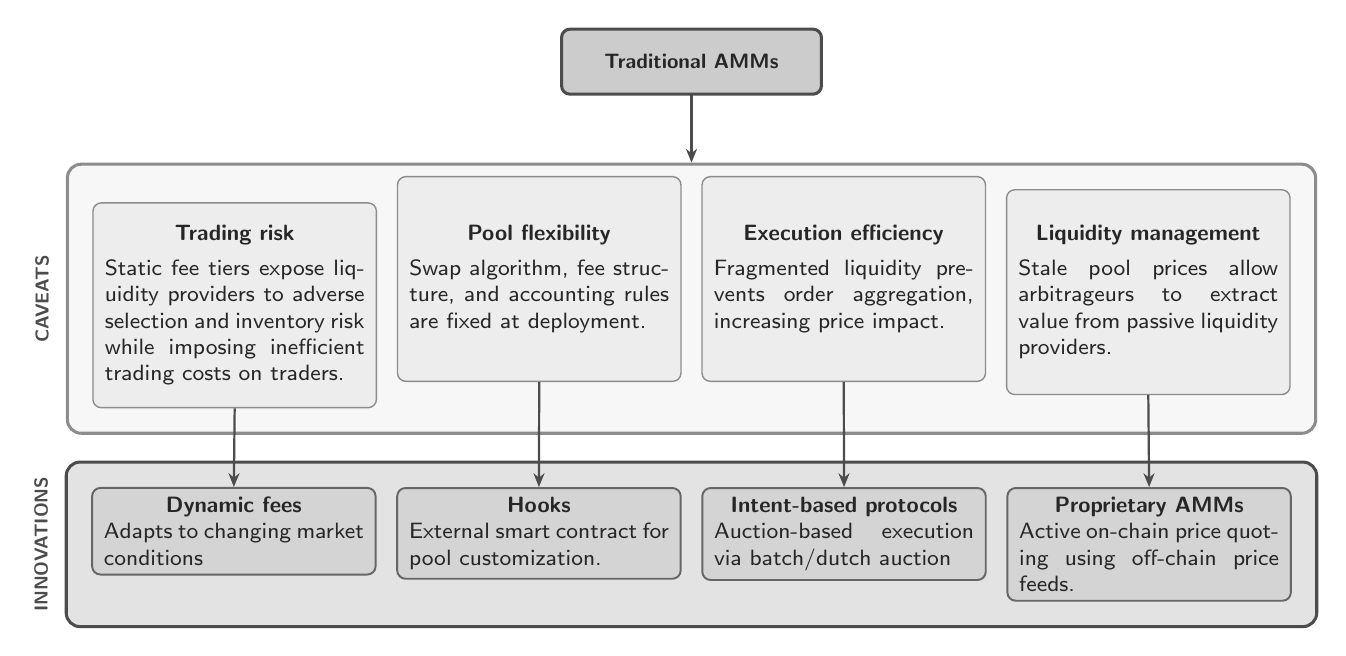
\begin{tikzpicture}[
  scale=0.75,
  node distance=0.45cm and 0.45cm,
  every node/.style={transform shape}
]

% --- Greyscale palette ---
\definecolor{gsOuterCav}{gray}{0.97}
\definecolor{gsInnerCav}{gray}{0.93}
\definecolor{gsOuterSol}{gray}{0.89}
\definecolor{gsInnerSol}{gray}{0.83}
\definecolor{gsRoot}{gray}{0.80}
\definecolor{gs30}{gray}{0.30}
\definecolor{gs55}{gray}{0.55}
\definecolor{gs40}{gray}{0.40}
\definecolor{gs15}{gray}{0.15}

% --- Styles ---
\tikzset{
  base/.style={
    rectangle, rounded corners=3pt,
    align=justify,
    font=\footnotesize\sffamily,
    text=gs15,
    execute at begin node=\setlength{\parindent}{0pt}\setlength{\parskip}{0pt}
  },
  rootnode/.style={base, minimum width=4.4cm, minimum height=1.1cm,
                fill=gsRoot, draw=gs30, line width=1.1pt,
                font=\normalsize\bfseries\sffamily},
  caveatnode/.style={base, minimum width=3.6cm, minimum height=2.6cm,
                text width=3.3cm,
                fill=gsInnerCav, draw=gs55, line width=0.5pt},
  solnode/.style={base, minimum width=3.6cm, minimum height=1.1cm,
                text width=3.3cm,
                fill=gsInnerSol, draw=gs40, line width=0.7pt},
  myarrow/.style={-{Stealth[length=5pt, width=4pt]}, line width=0.8pt, color=gs30},
  outerlabel/.style={font=\small\bfseries\sffamily, text=gs30, rotate=90, anchor=center}
}

% --- Caveats (as a matrix for clean alignment) ---
\matrix (cav) [matrix of nodes, row sep=0pt, column sep=2.5mm, nodes={caveatnode}] {
  {{\centering\textbf{Trading risk}\par}\smallskip\justifying \noindent Static fee tiers expose liquidity providers to adverse selection and inventory risk while imposing inefficient trading costs on traders.} &
  {{\centering\textbf{Pool flexibility}\par}\smallskip\justifying
  \noindent Swap algorithm, fee structure, and accounting rules are fixed at deployment.} &
  {{\centering\textbf{Execution efficiency}\par}\smallskip\justifying
  \noindent Fragmented liquidity prevents order aggregation, increasing price impact.} &
  {{\centering\textbf{Liquidity management}\par}\smallskip\justifying
  \noindent Stale pool prices allow arbitrageurs to extract value from passive liquidity providers.} \\
};

% --- Root node (centered above caveats) ---
\node[rootnode, above=12mm of cav] (root) {Traditional AMMs};

% --- Outer CAVEATS box ---
\begin{scope}[on background layer]
  \node[fill=gsOuterCav, draw=gs55, line width=1.1pt, rounded corners=5pt,
        fit=(cav-1-1)(cav-1-4), inner sep=9pt] (caveatbox) {};
\end{scope}

% --- Innovations (matrix aligned with caveats) ---
\matrix (sol) [matrix of nodes, below=10mm of cav, row sep=0pt, column sep=2.5mm, nodes={solnode}] {
  {{\centering\textbf{Dynamic fees}\par}\footnotesize\justifying\noindent Adapts to changing market conditions} &
  {{\centering\textbf{Hooks}\par}\footnotesize\justifying \noindent External smart contract for pool customization.} &
  {{\centering\textbf{Intent-based protocols}\par}\footnotesize\justifying
  \noindent Auction-based execution via batch/dutch auction} &
  {{\centering\textbf{Proprietary AMMs}\par}\footnotesize\justifying \noindent Active on-chain price quoting using off-chain price feeds.} \\
};


% --- Outer INNOVATIONS box ---
\begin{scope}[on background layer]
  \node[fill=gsOuterSol, draw=gs30, line width=1.1pt, rounded corners=5pt,
        fit=(sol-1-1)(sol-1-4), inner sep=9pt] (solbox) {};
\end{scope}

% --- Left-side rotated labels (centered on the boxes) ---
\node[outerlabel] at ([xshift=-4.0mm]caveatbox.west) {CAVEATS};
\node[outerlabel] at ([xshift=-4.0mm]solbox.west) {INNOVATIONS};

% --- Arrows ---
\draw[myarrow] (root.south) -- (caveatbox.north);
\draw[myarrow] (cav-1-1.south) -- (sol-1-1.north);
\draw[myarrow] (cav-1-2.south) -- (sol-1-2.north);
\draw[myarrow] (cav-1-3.south) -- (sol-1-3.north);
\draw[myarrow] (cav-1-4.south) -- (sol-1-4.north);

\end{tikzpicture}

\end{document}

